\documentclass[a4paper]{article}
\usepackage[T1]{fontenc}
\usepackage[margin=1in]{geometry}
\usepackage{listings}
\usepackage{xcolor}
\usepackage{courier}
\usepackage{graphicx}
\usepackage{hyperref}
\usepackage{sidecap}
\usepackage{wrapfig}
\usepackage{subfig}
\usepackage{float}
\renewcommand{\figurename}{Rysunek}

\lstdefinestyle{sharpc}{language=[Sharp]C, frame=lr, rulecolor=\color{blue!80!black}}

\title{Analiza częstotliwościowa sygnału audio\\
\large Projekt nr 2 - Analiza i Przetwarzanie Dźwięku\\ 
\small \url{https://github.com/szymon159/sound-analysis}}
\date{}
\author{Szymon Stasiak}

\begin{document}
  \maketitle

\section{Opis aplikacji}
Projekt stworzony został w .NET Framework, z warstwą prezentacji powstałą w Windows Forms i interfejsem w języku angielskim. Analiza wspiera pliki \textit{*.wav} oraz \textit{*.mp3}.\\
Jest to rozwinięcie projektu \textit{Cechy sygnału audio w dziedzinie czasu}, dodające do poprzedniej wersji 3 nowe opcje widoku - widmo częstotliwościowe, spektrogram oraz wykres częstotliwości tonu podstawowego.\\
W celu uproszczenia obliczeń dodane zostały również referencje do paczek:
\begin{itemize}
\item \textit{NAudio} (w celu wczytywania, parsowania i podstawowych operacji na plikach)
\item \textit{MathNet.Numerics} - dostarcza narzędzia do obliczania transformaty Fouriera oraz stosowania funkcji okienkowych
\item \textit{Oxyplot} - usprawnienie wykresów
\end{itemize}

\subsection{Głowne okno programu}
Główne okno programu uległo nieznacznej zmianie w stosunku do poprzedniej części projektu.\\
Główna część (tj. wartości i wykresy obliczanych parametrów) znajdują się obecnie w odpowiednich zakładkach - zakładka \textit{Time Parameters} odpowiada \textit{Projektowi 1}, natomiast kolejne zakładki - \textit{Fourier Transform}, \textit{Spectrogram} oraz \textit{Fundamental Frequency} odpowiadają nowo zaimplementowanym funkcjom.\\
Ponadto obok wykresu utworu w dziedzinie czasu dodana została możliwość wyboru okna - dostępna wyłącznie dla nowych funkcji.
\begin{figure}[H]
  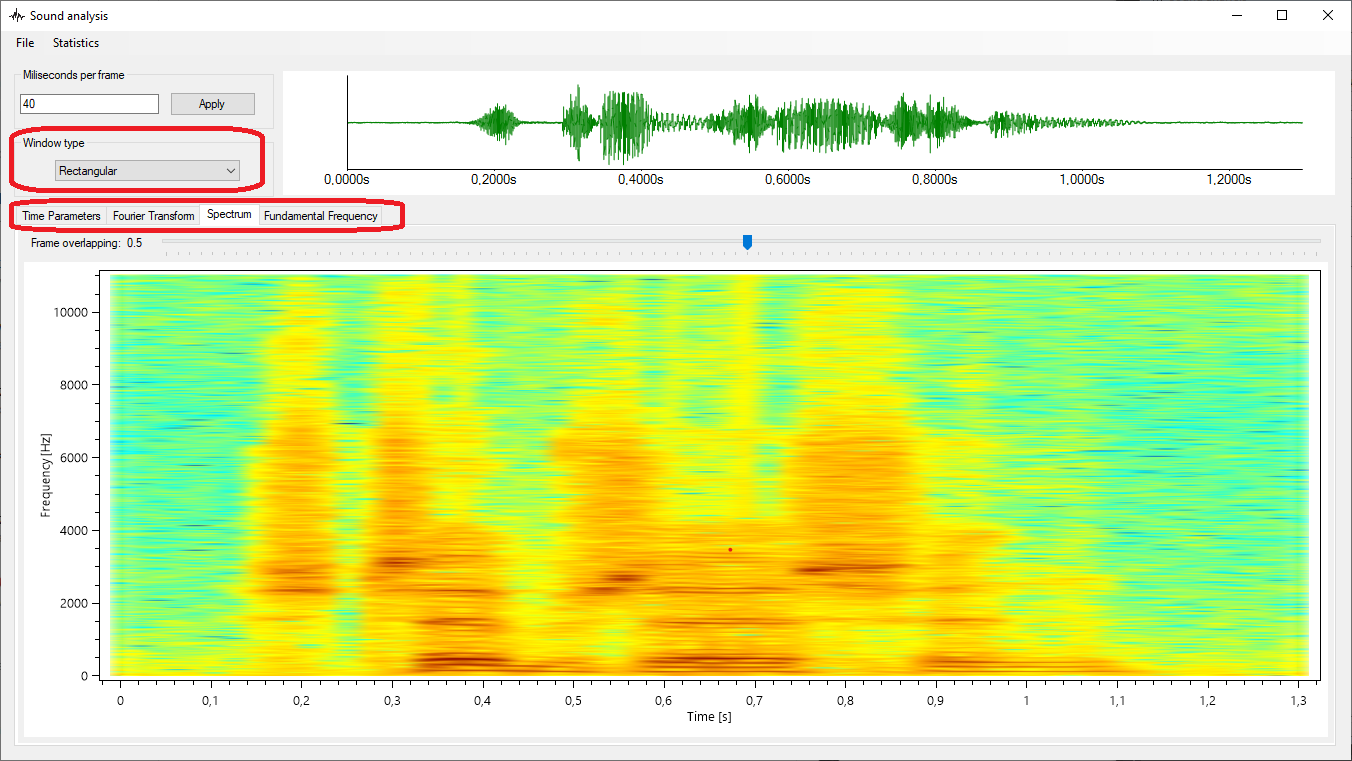
\includegraphics[width=\linewidth]{images/01interface.png}
  \caption{Interfejs programu z zaznaczonymi nowymi opcjami}
\end{figure}

\section{Opis metod}
\subsection{Analiza w dziedzinie częstotliwości (\textit{Fourier Transform})}
Używana nazwa tej sekcji (Fourier Transform) wywodzi się od metody wykorzystywanej w celu przejścia z dziedziny czasu do dziedziny częstotliwości.\\
Gwoli ścisłości - użyty został algorytm \textit{Fast Fourier Transform} wyznaczający wynik dyskretnej transformaty Fouriera.\\
Z pomocą przyszła tutaj implementacja metody \textit{Fourier.Forward} z biblioteki \textit{MathNet.Numerics}. Wartości widoczne na wykresach przedstawiają (odpowiednio przeskalowany) logarytm dziesiętny z modułu wartości transformacji dla danej próbki.\\
Warto wspomnieć, iż dyskretna transformata Fouriera zdefiniowana jest dla ilości punktów będącej potęgą liczby $2$. W celu spełnienia tego wymagania, analizowane nagranie zostało rozszerzone do najbliższej potęgi próbkami o wartości równej $0$. Próbki te nie prezentują żadnego dźwięku, toteż nie wpływają one destrukcyjnie na kształt samego wykresu.\\
Kolejnym ważnym aspektem jest \textit{częstotliwość Nyquista}. Mianem tym określana jest własność wynikająca z \textit{twierdzenia o próbkowaniu} zwanego także \textit{twierdzeniem Nyquista-Shannona}. Zgodnie z tym twierdzeniem, wyniki analizy częstotliwościowej są symetryczne dla niskich oraz wysokich częstotliwości. Mówiąc dokładniej, wyznaczając wartości można ograniczyć się przez wartość $\frac{f_0}{2}$ gdzie $f_0$ oznacza częstotliwość próbkowania.\\
Z tego powodu na poniższych wykresach dla nagrania o częstotliwości próbkowania $f_0 = 22 050Hz$ wartości na osi OX przedstawione są wyłącznie w zakresie $[0, 11 025Hz]$.
\begin{figure}[H]
  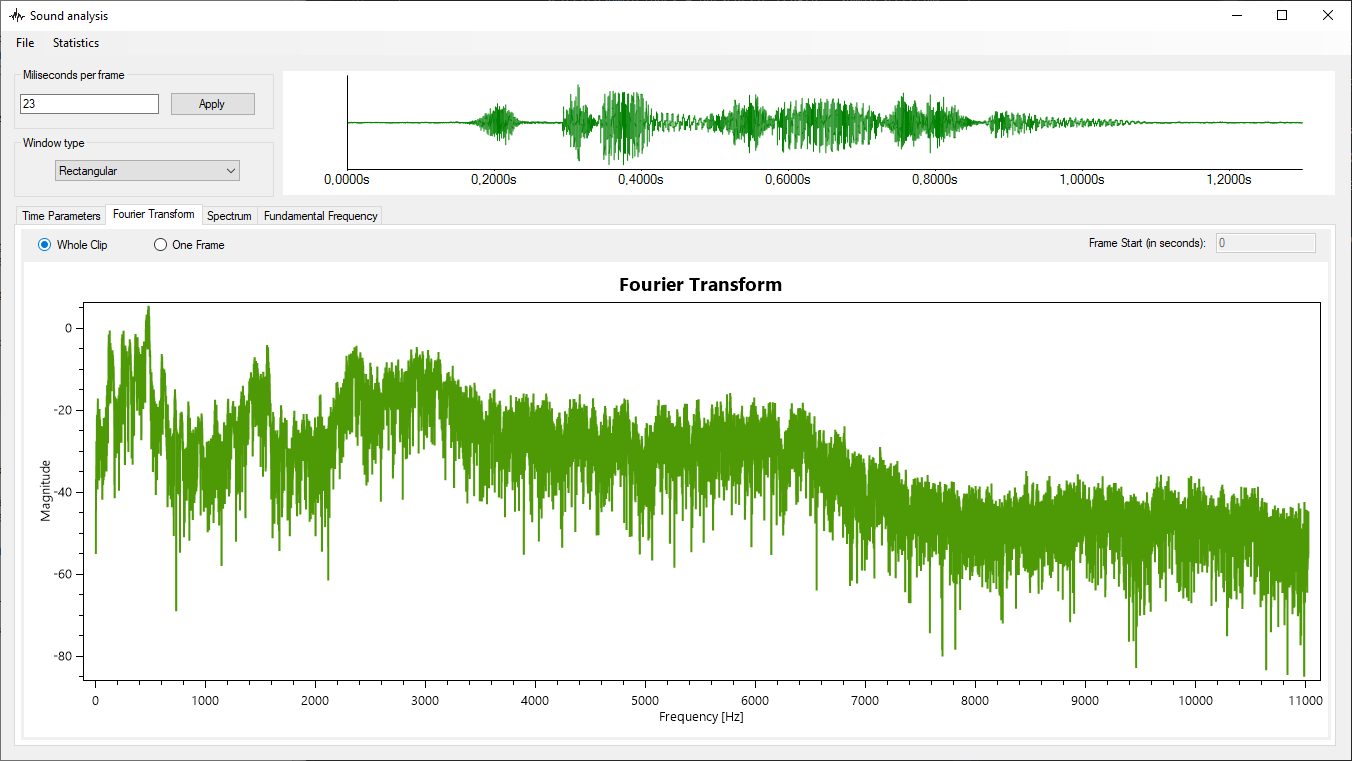
\includegraphics[width=\linewidth]{images/02fourier.png}
  \caption{Przykładowe nagranie w dziedzinie częstotliwości}
\end{figure}
Podobnie wygląda sytuacja w przypadku analizy jednej próbki. W tym przypadku analiza dotyczy fragmentu nagrania o długości zależnej od podanych wartości \textit{Miliseconds per frame} oraz \textit{Frame Start}. Długość ramki w milisekundach jest wówczas konwertowana na odpowiadającą jej ilość próbek w jednej ramce. A następnie wybrane próbki zostają rozszerzone do najbliższej potęgi liczby $2$.\\
Przykładowa analiza dla jednej ramki powyższego nagrania przedstawiona została na \textit{Rysunku 3} dostępnym na następnej stronie.
\begin{figure}[H]
  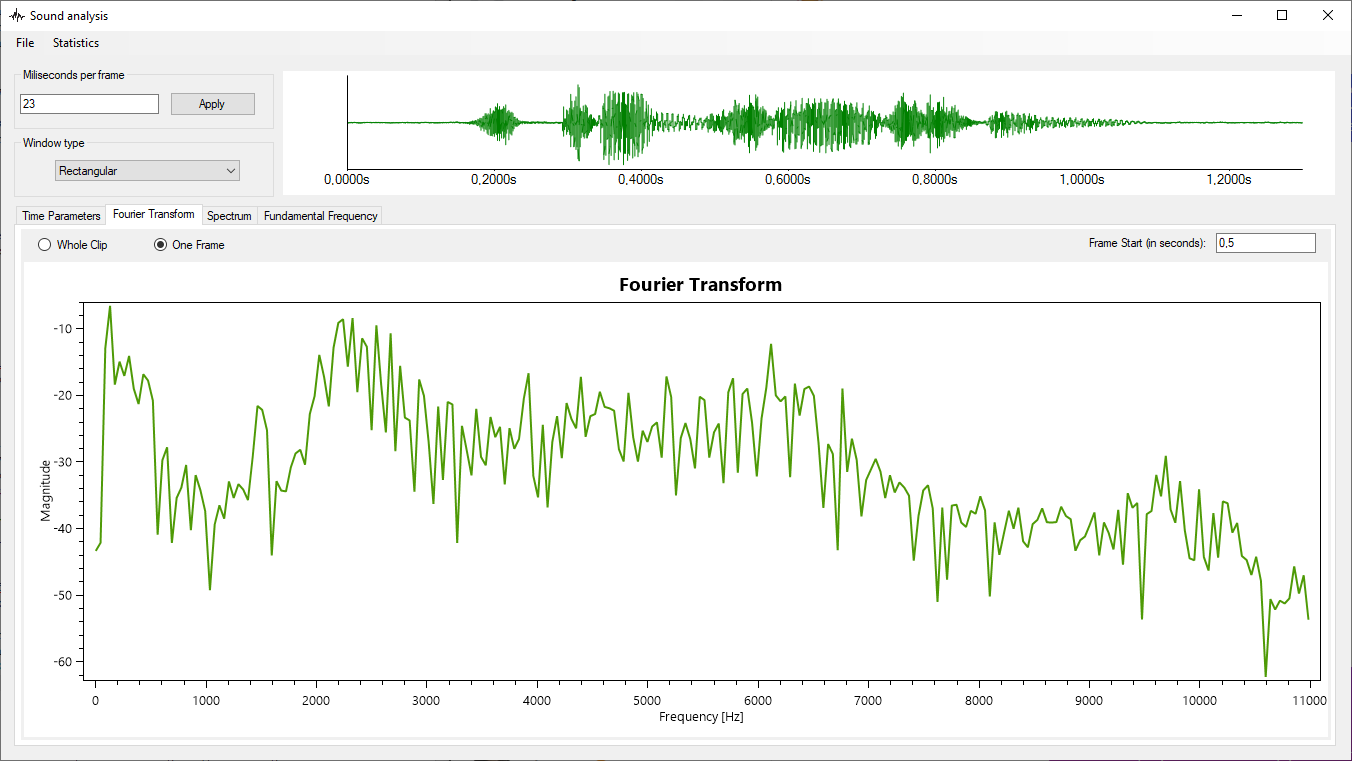
\includegraphics[width=\linewidth]{images/03fourierInFrame.png}
  \caption{Fragment nagrania przedstawiony w dziedzinie częstotliwości}
\end{figure}

\subsection{Analiza widmowa (\textit{Spectrogram})}
\begin{figure}[H]
  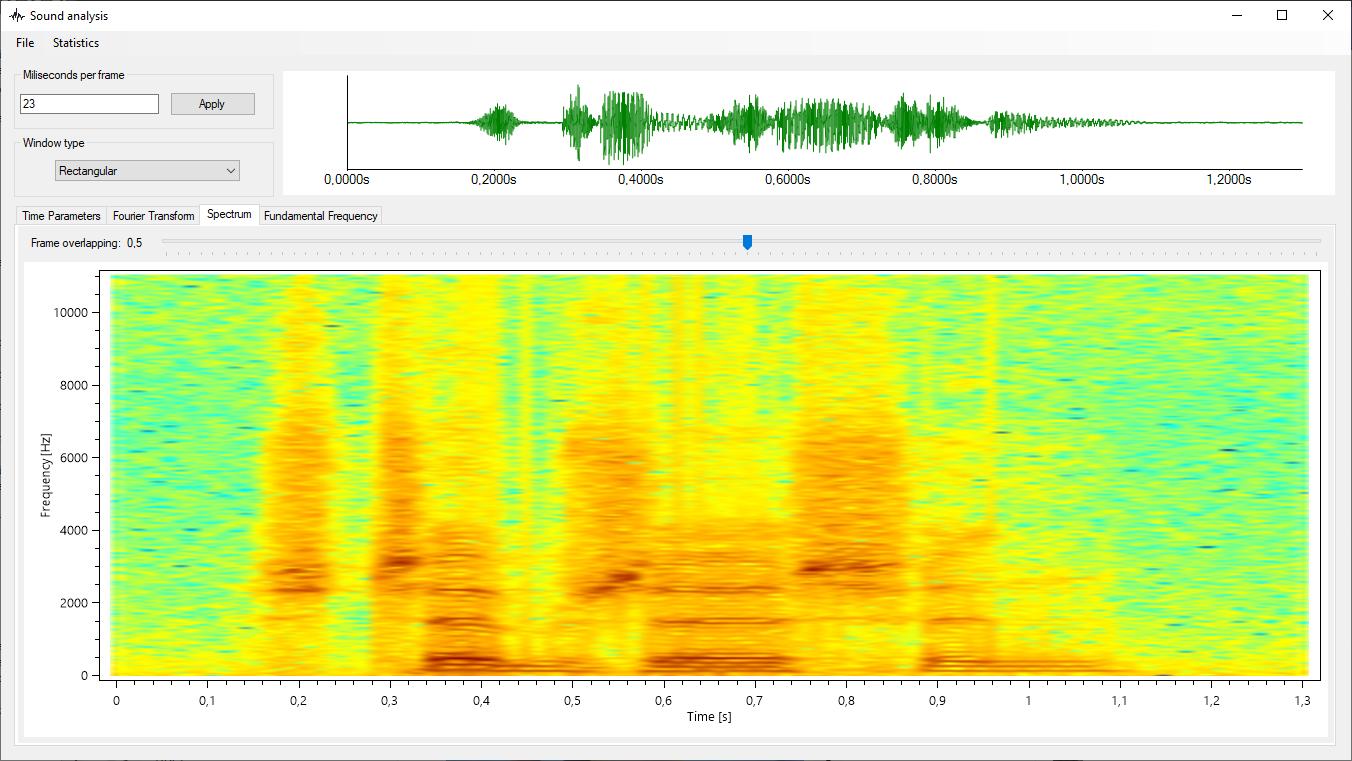
\includegraphics[width=\linewidth]{images/04spectrogram.png}
  \caption{Spektrogram dla przykładowego nagrania (wartość nakładania ramek $l=0.5$)}
\end{figure}
W celu uzyskania spektrogramu należy podzielić całe nagranie na ramki odpowiadające przedziałom czasowym a następnie dla każdej takiej ramki wyznaczyć wynik \textit{dyskretnej transformaty Fouriera}.\\
Ważnym parametrem przy analizie spektralnej jest \textit{nakładanie się ramek} (\textit{frame overlapping}). Jest to parametr z przedziału $(0, 1)$ określający jaki fragment (licząc w próbkach) jest wspólny dla dwóch sąsiadujących ramek.\\
Transformata Fouriera jest obarczona pewną niedokładnością na skrajach przedziałów. Z tego powodu, dla małych ramek, informacja na ich skrajach może być utracona bądź zdeformowana. Aby zminimalizować to zjawisko sąsiednie ramki mogą się na siebie nakładać. Graficznie widoczne jest to przede wszystkim poprzez różnicę w ostrości wykresów.\\
Powyższy \textit{Rysunek 4} przedstawia wykres dla wartości nakładania się ramek równej $l = 0.5$ natomiast poniższe: \textit{Rysunek 5} oraz \textit{Rysunek 6} - spektrogramy dla wartości równych odpowiednio: $l_1 = 0.01$ oraz $l_2 = 0.99$:
\begin{figure}[H]
  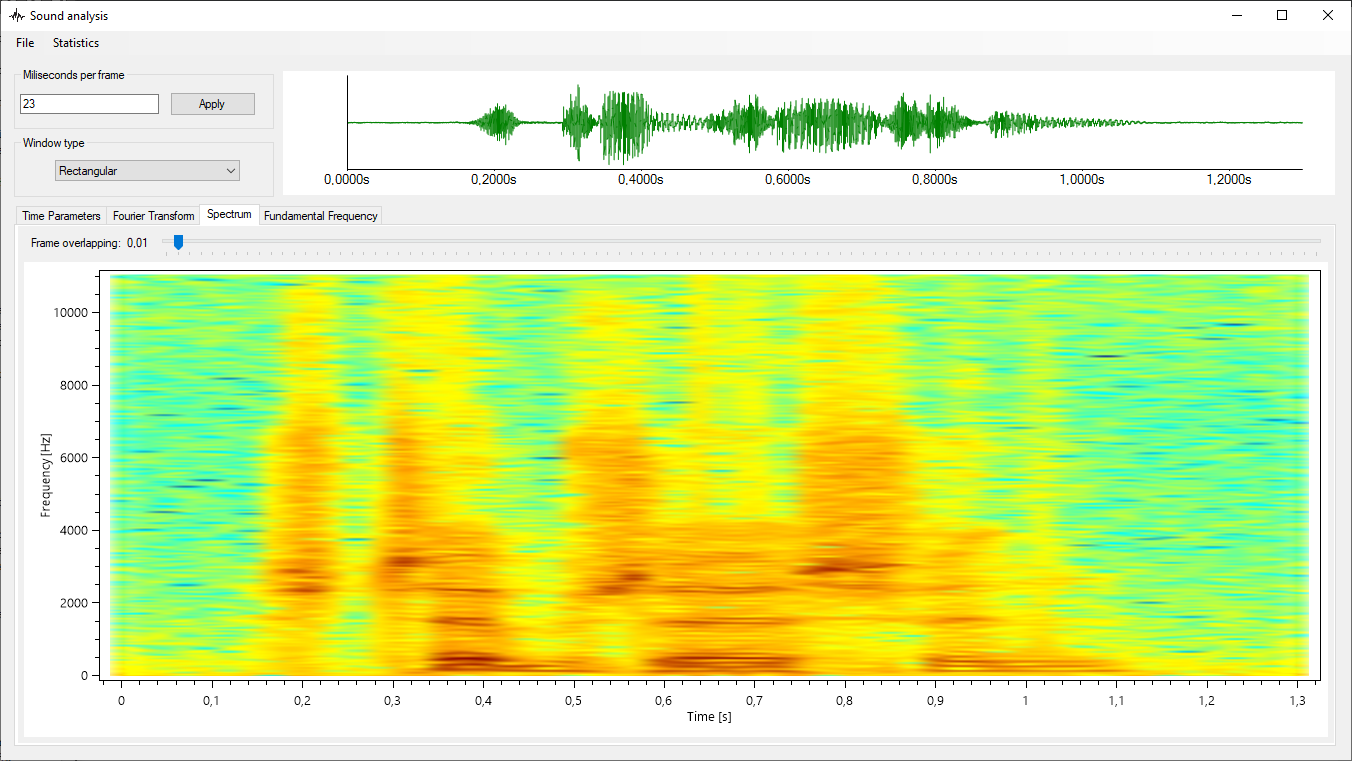
\includegraphics[width=\linewidth]{images/05spectrogramLowOverlap.png}
  \caption{Spektrogram dla przykładowego nagrania (wartość nakładania ramek $l=0.01$)}
\end{figure}
\begin{figure}[H]
  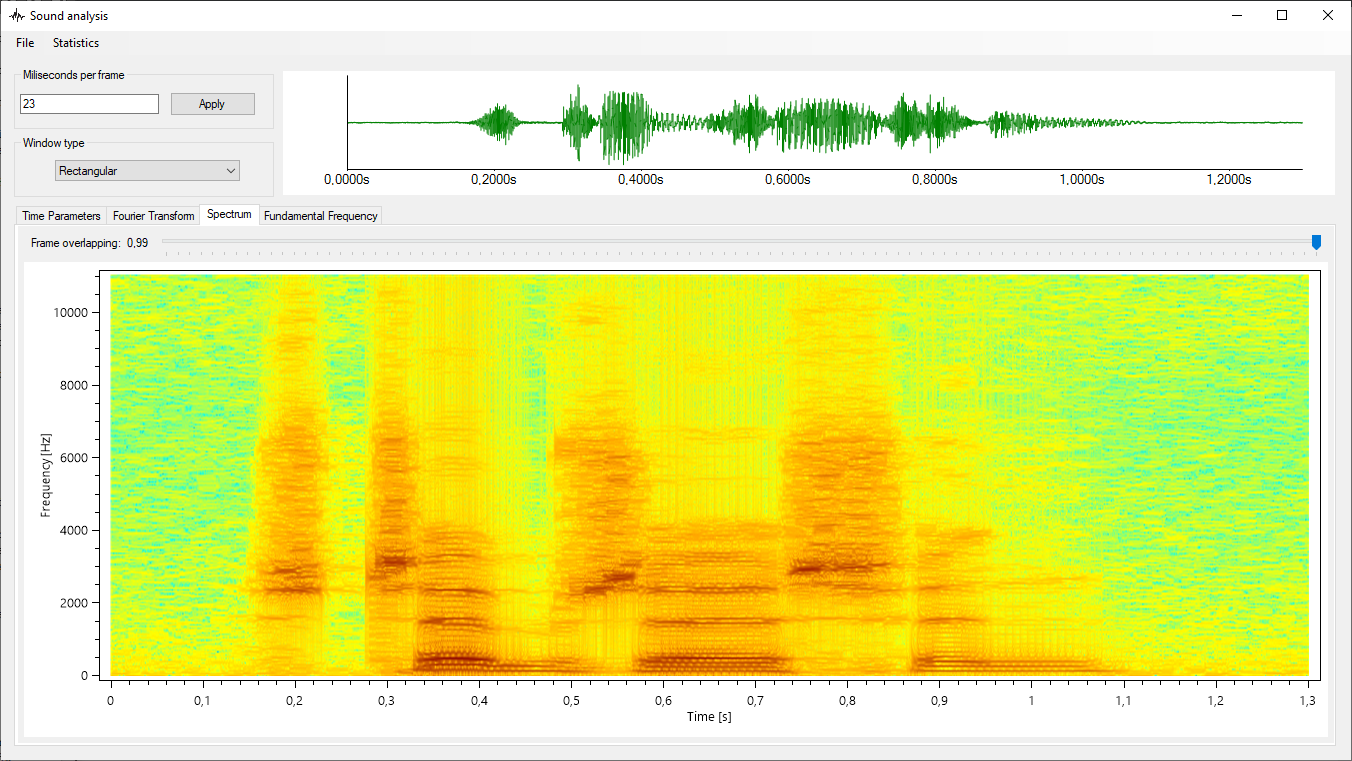
\includegraphics[width=\linewidth]{images/06spectrogramHighOverlap.png}
  \caption{Spektrogram dla przykładowego nagrania (wartość nakładania ramek $l=0.99$)}
\end{figure}

Z pewnością wyniki działania tej metody należą do najefektowniejszych. Nie można im również odmówić przydatności.\\
Korzystając z wykresu w poprzedniej sekcji można określić jakie częstotliwości dominują w nagraniu. Najwyższe wartości są bowiem osiągane dla częstotliwości w okolicach $100 - 500Hz$, co nie jest niespodzianką gdyż nagranie przedstawia fragment mowy. Nie mamy jednak możliwości detekcji w których momentach mowa ustępuje miejsca ciszy, co było proste do określenia z wykresu w dziedzinie czasu.\\
W tym celu używany jest spektrogram, gdzie oś pionowa przedstawia częstotliwość, pozioma - czas, zaś natężenie barwy odpowiada natężeniu dźwięku.
Widoczny na trzech powyższych rysunkach spektrogram odpowiada nagraniu analizowanemu również w poprzednich sekcjach. Łatwo więc zauważyć że i tutaj największe natężenie przypada na dźwięki poniżej $1000 Hz$. Jednak dzięki zawarciu informacji o czasie, wyniki działania spektrogramu można również porównywać z wykresem w dziedzinie czasu - otrzymujemy możliwość określenia przedziałów ciszy oraz największego natężenia dźwięku.\\

\subsection{Częstotliwość tonu podstawowego (\textit{Fundamental Frequency})}
Jedną z często używanych wartości wyznaczanych w wyniku operacji na fali dźwiękowej jest częstotliwość tonu podstawowego. Jest to wartość używana szczególnie w przypadku analizy krótkich dźwięków czy fragmentów muzyki. Nawet czysty dźwięk instrumentu muzycznego nastrojonego na daną częstotliwość jest tak naprawdę złożeniem kilku fal dźwiękowych o częstotliwościach będących wielokrotnością częstotliwości tonu podstawowego.\\
Wartość ta jest jednak określana również w przypadku mowy. Oznacza ona wówczas składową częstotliwość tonu krtaniowego, a więc dźwięku powstającego w krtani podczas wymowy konkretnej głoski.\\
W celu wyznaczenia jej wartości należy zacząć od przekształcenia każdej kolejnej ramki (dobieranej analogicznie do spektrogramu) z użyciem dyskretnej transformaty Fouriera. Jednak w wyniku tej operacji otrzymujemy wartości w dziedzinie częstotliwości, zaś interesująca nas wartość wyznaczana jest w dziedzinie czasu. Z tego powodu należy poddać otrzymane wartości \textit{odwrotnej transformacji Fouriera}. Argument dla którego osiągane jest lokalne maksimum rzeczywiste dźwięku określa wówczas poszukiwaną częstotliwość.\\
Należy jednak pamiętać w jakim przedziale warto szukać owego lokalnego maksimum - w przypadku mowy wystarczy ograniczyć się do przedziału $[50, 400] Hz$. Wartości spoza tego zakresu to zazwyczaj szumy bądź dźwięki tła które nie powinny mieć wpływu na analizę.\\
Poniższy \textit{Rysunek 7} przedstawia właśnie wykres częstotliwości tonu podstawowego dla nagrania mowy - jak widać częstotliwości całego fragmentu oscylują wokół podobnych wartości.
\begin{figure}[H]
  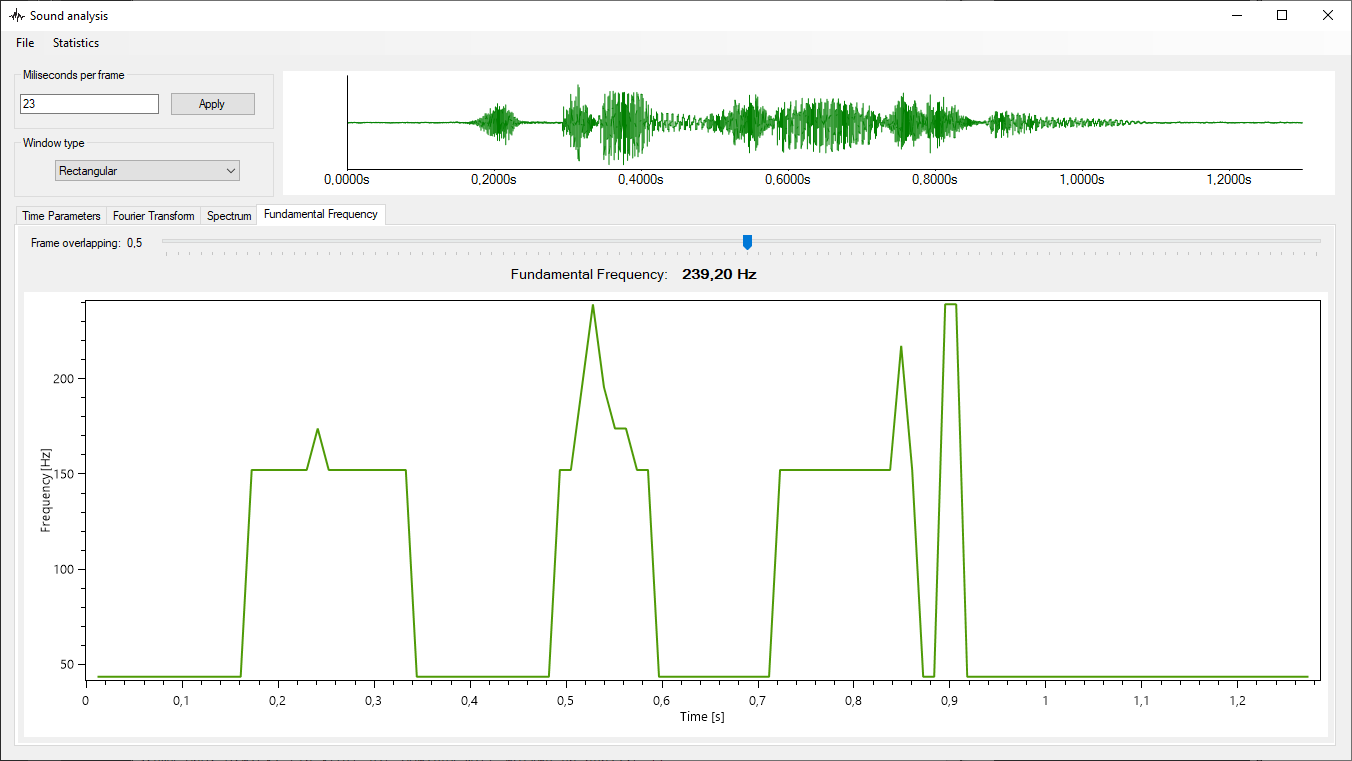
\includegraphics[width=\linewidth]{images/07fundamentalFrequency.png}
  \caption{Częstotliwość tonu podstawowego}
\end{figure}

\section{Wyniki działania}
\subsection{Funkcje okienkowe}
Analizując wyniki działania poszczególnych metod warto poświęcić chwilę na analizę różnic wynikających z zastosowanych \textit{funkcji okienkowych}. Różnice te są szczególnie widoczne w przypadku spektrogramu.\\
W przypadku okna prostokątnego brakuje wyraźnego odróżnienia fragmentów mowy oraz szumu. Dźwięki o częstotliwościach niedominujących osiągają podobne natężenie zarówno w momentach ciszy jak i mowy. Ciemniejsze słupki częstotliwości dominujących zdają się znajdować na tle niemal jednolitym (bez różnicy czy patrzymy na skraj czy też środek nagrania).
\begin{figure}[H]
  \centering  
  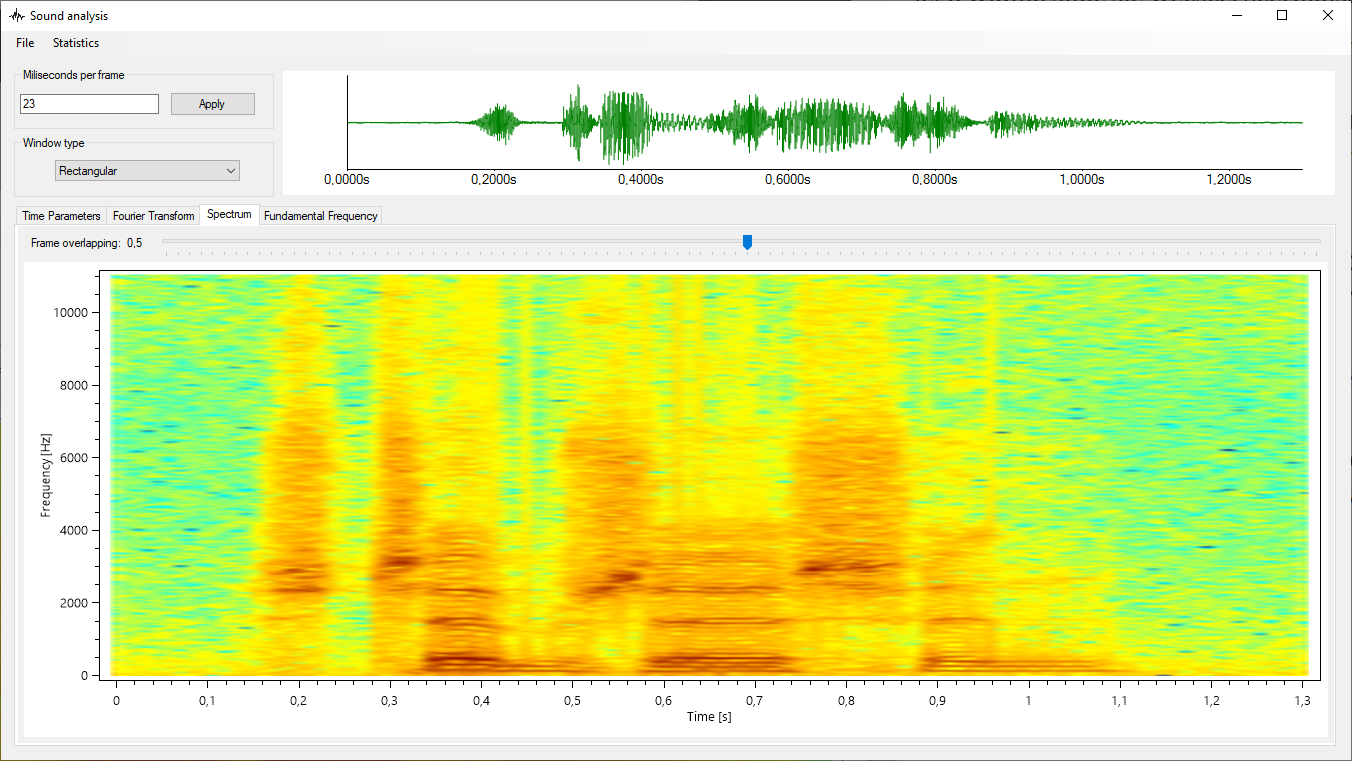
\includegraphics[width=0.86\linewidth]{images/08rectangularWindow.png}
  \caption{Spektrogram dla okna prostokątnego}
\end{figure}
Inaczej wygląda sytuacja w przypadku zastosowania okna Hanna (\textit{Rysunek 9}).\\
Fragmenty skrajne (a więc pozbawione mowy) wyraźnie odznaczają się od części centralnej. Z drugiej strony, precyzyjne wyznaczenie "słupków" dominujących częstotliwości jest bardziej skomplikowane - nie odróżniają się one tak widocznie od tła.
\begin{figure}[H]
  \centering
  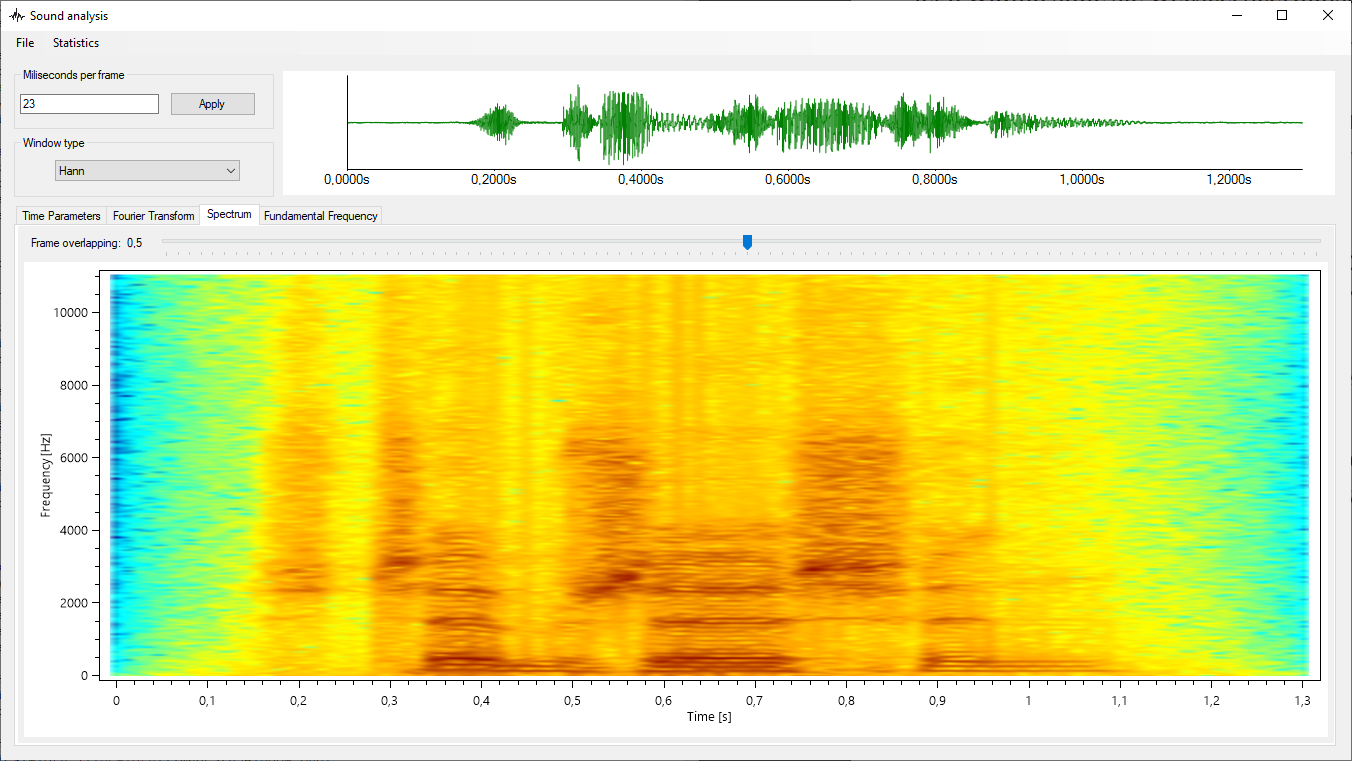
\includegraphics[width=0.86\linewidth]{images/09hannWindow.png}
  \caption{Spektrogram dla okna Hanna}
\end{figure}

\subsection{Porównanie mowy dwóch osób}
Kolejnym aspektem poddanym analizie jest porównanie głosu dwóch osób. W tym celu, porównaniu zostały poddane nagrania tego samego słowa - "Szczebrzeszyn" w wykonaniu moim oraz mojego brata - Pawła. Wiele osób twierdzi iż głosy te są bardzo podobne (a pomylone imię w czasie rozmowy telefonicznej to już standard). W celu zminimalizowania różnic, oba nagrania używają tylko jednego kanału, ponadto zostały one poddane normalizacji. Częstotliwość próbkowania wynosi w obu przypadkach $22050 Hz$.\\
Zgodnie z przewidywaniami, różnice w wyniku transformaty Fouriera są widoczne, jednak nie można ich powiązać bezpośrednio z cechami głosu autora. Powstałe tutaj różnice mogą wynikać z różnicy w intonacji, akcencie. Poniższe rysunki przedstawiają wykresy w dziedzinie częstotliwości dla nagrań odpowiednio - mojego oraz Pawła.\\
Różnice w przedziale $[50, 400 Hz]$ są wręcz pomijalne.
\begin{figure}[H]
  \centering
  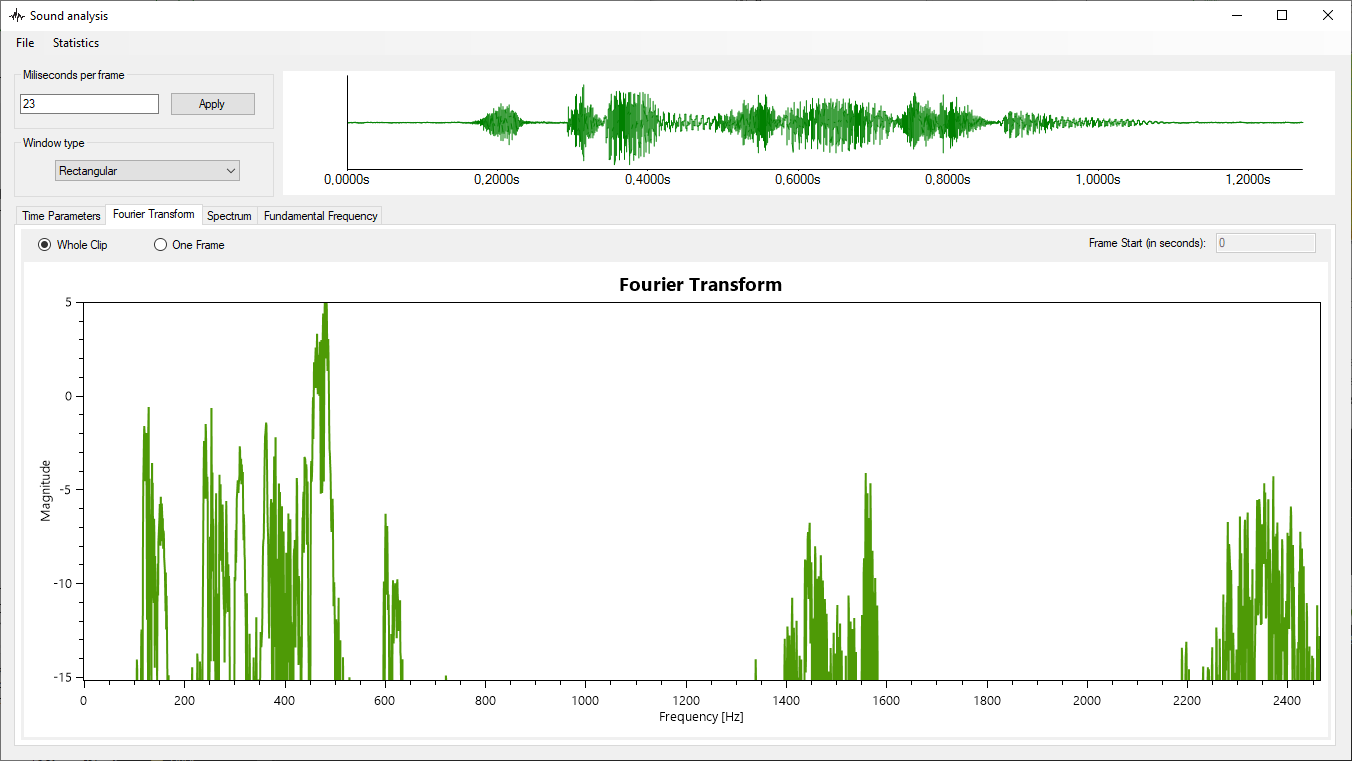
\includegraphics[width=0.86\linewidth]{images/10fourierMy.png}
  \caption{Transformata Fouriera dla mojego nagrania}
\end{figure}
\begin{figure}[H]
  \centering
  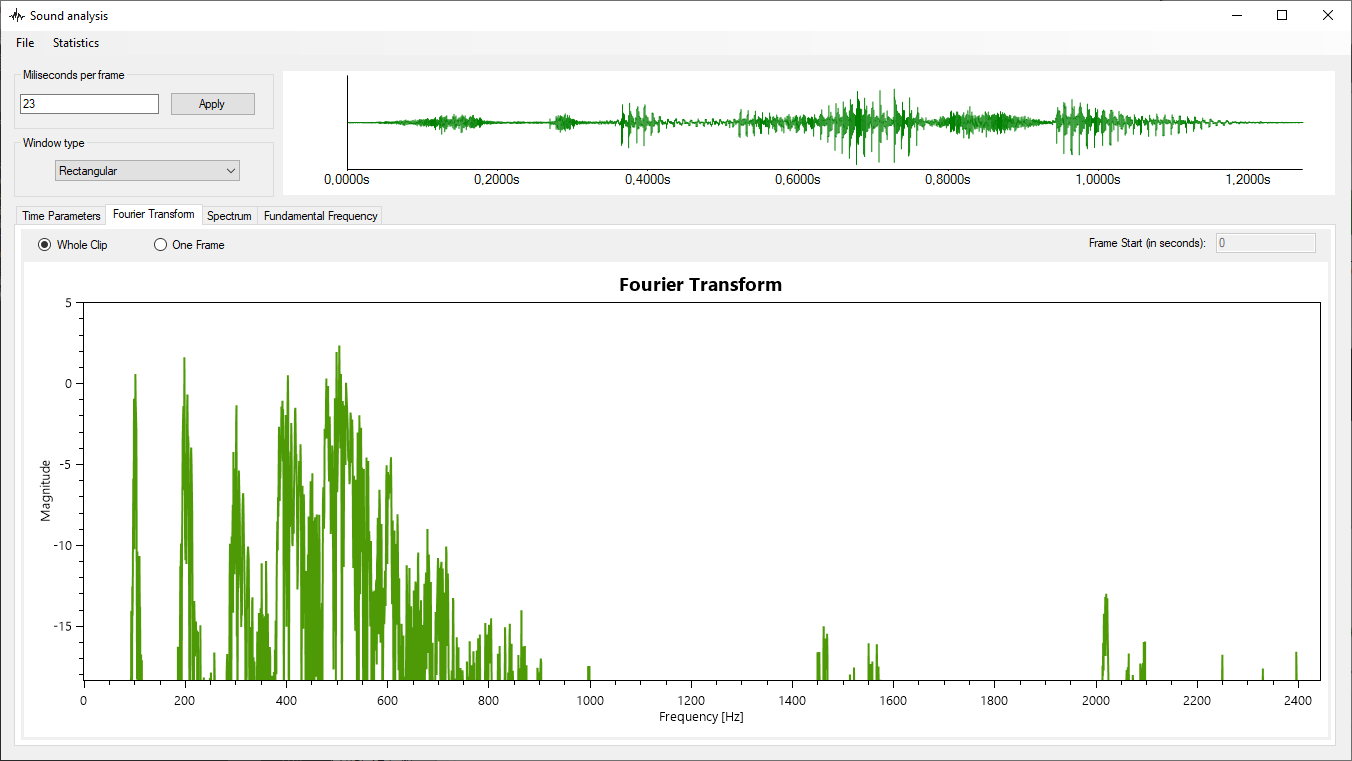
\includegraphics[width=0.86\linewidth]{images/11fourierBro.png}
  \caption{Transformata Fouriera dla nagrania Pawła}
\end{figure}
Sytuacja wygląda podobnie w przypadku analizy widmowej. Nie jest to jednak zaskakujące, gdyż analiza ta dokładniej przedstawia samą dynamikę nagrania.\\
Widać jednak różnicę powiązaną w mniejszym stopni z samym głosem - jest to szybkość mówienia. Jak widać na poniższych rysunkach, większość fragmentów zawierających mowę znajduje się w centralnej części spektrogramu dla mojego nagrania, zaś w przypadku nagrania Pawła fragment ten jest bardziej rozciągnięty.
\begin{figure}[H]
  \centering
  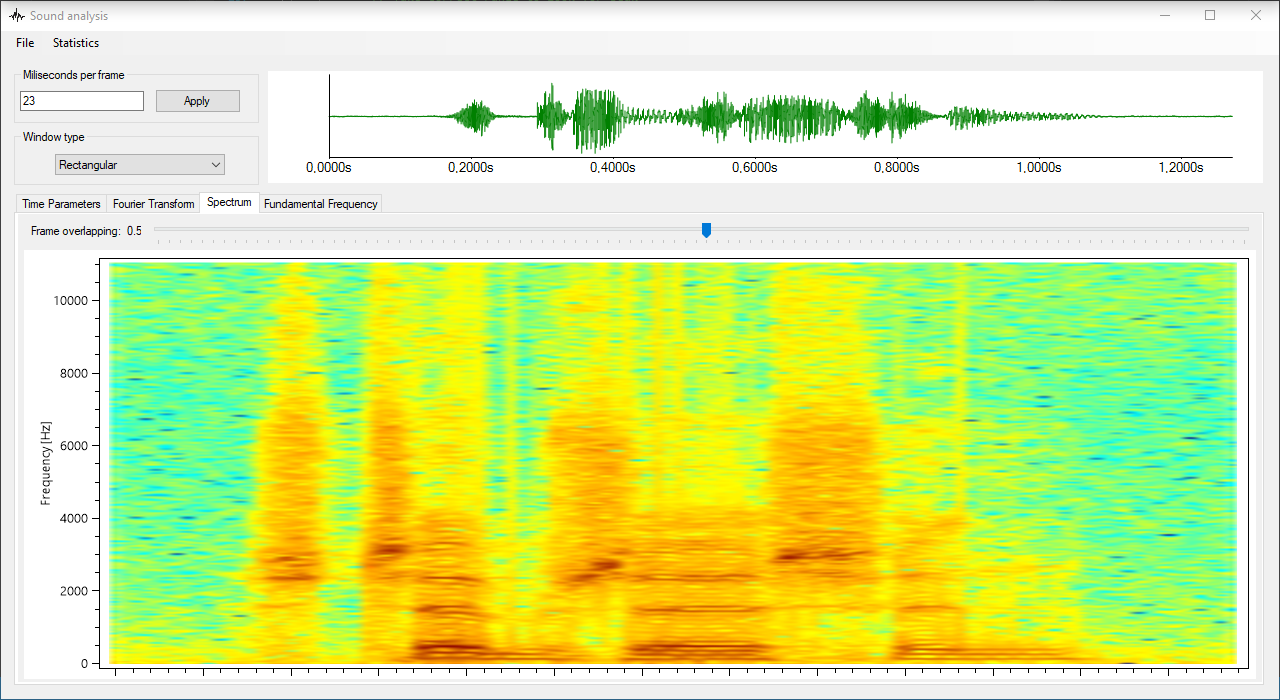
\includegraphics[width=0.86\linewidth]{images/12spectrogramMy.png}
  \caption{Transformata Fouriera dla mojego nagrania}
\end{figure}
\begin{figure}[H]
  \centering
  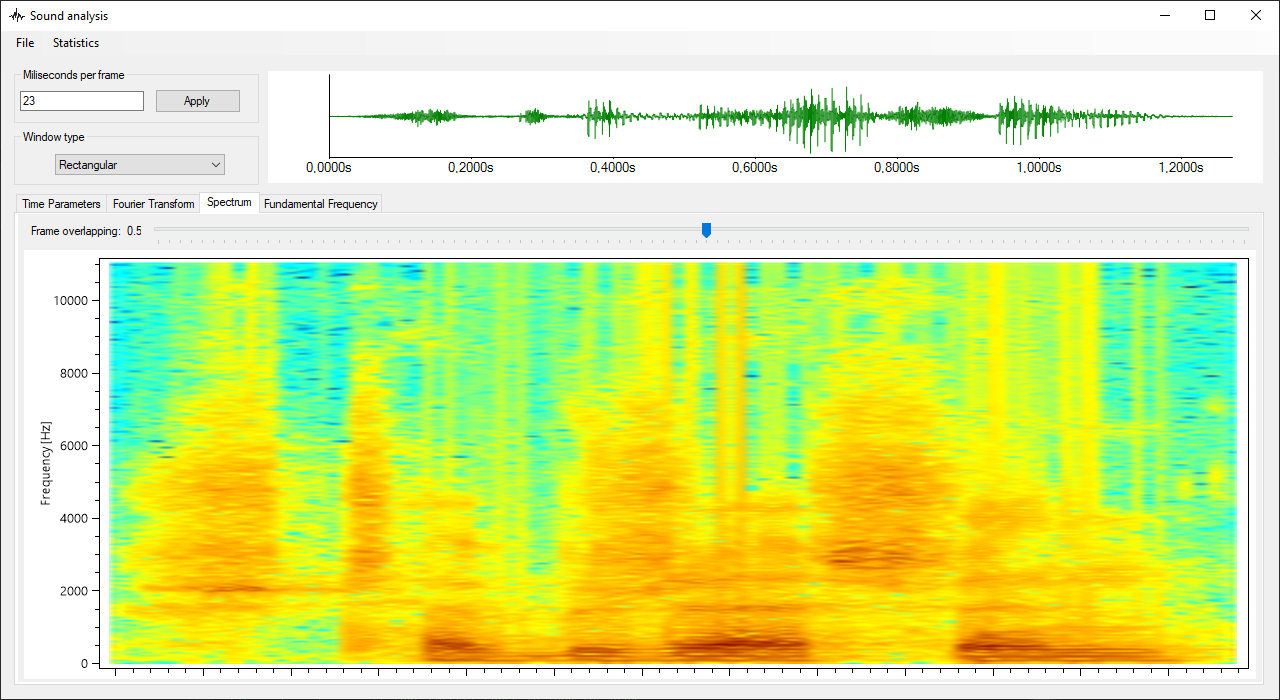
\includegraphics[width=0.86\linewidth]{images/13spectrogramBro.png}
  \caption{Transformata Fouriera dla nagrania Pawła}
\end{figure}
Największe, a zarazem najbardziej istotne różnice zaobserwować można w przypadku częstotliwości tonu podstawowego. O ile przesunięcie (rozciągnięcie) w czasie nie jest istotne, o tyle różnica w osiąganych częstotliwościach jest już interesująca.\\
Wartości osiągane przez nagranie autorstwa Pawła są znacznie wyższe co wskazuje na wyższą częstotliwość jego głosu w tym konkretnym nagraniu.\\
Ciekawe jest również rozłożenie szczytów na obu tych wykresach. W moim przypadku najwyższa część znajduje się w środku słowa, zaś w przypadku Pawła - na jego początku. Można na tej podstawie określić (skądinąd słusznie) iż w analizowanych nagraniach sposób wypowiadania słowa znacznie się różnił (chociażby pod kątem akcentu).\\Właśnie mnogość różnic sprawia, że wyniki tego eksperymentu warto brać "z przymrużeniem oka".
\begin{figure}[H]
  \centering
  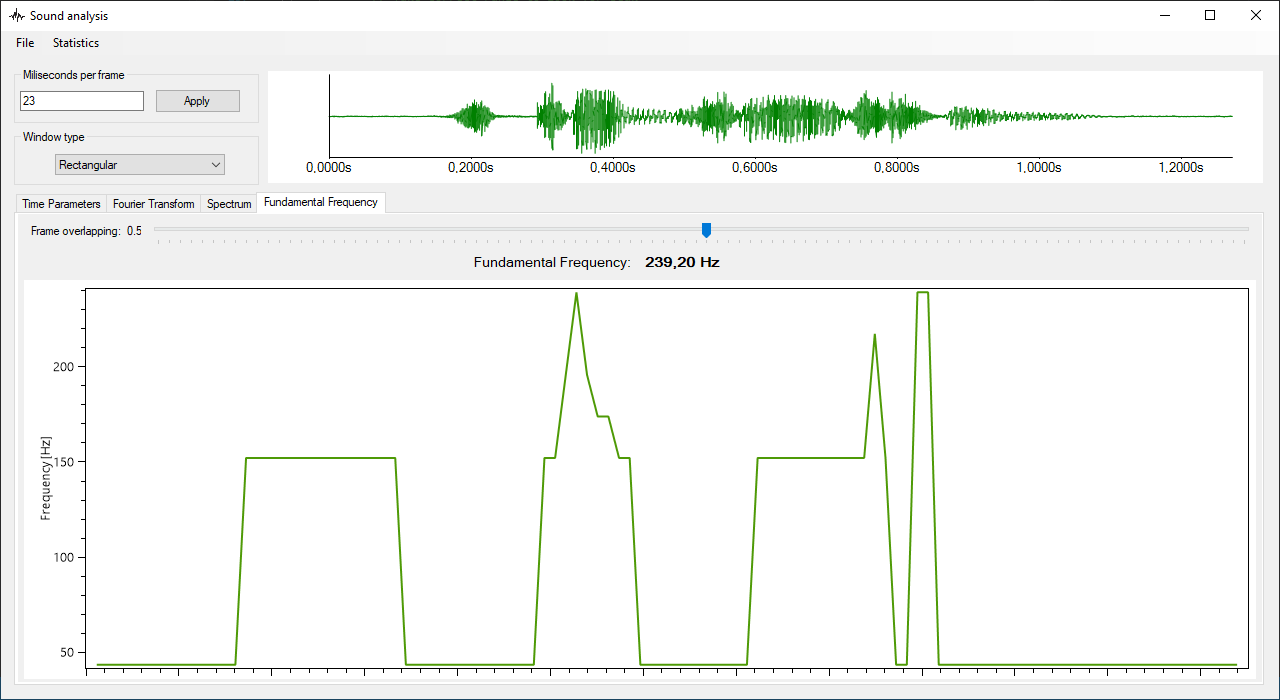
\includegraphics[width=0.86\linewidth]{images/14frequencyMy.png}
  \caption{Transformata Fouriera dla mojego nagrania}
\end{figure}
\begin{figure}[H]
  \centering
  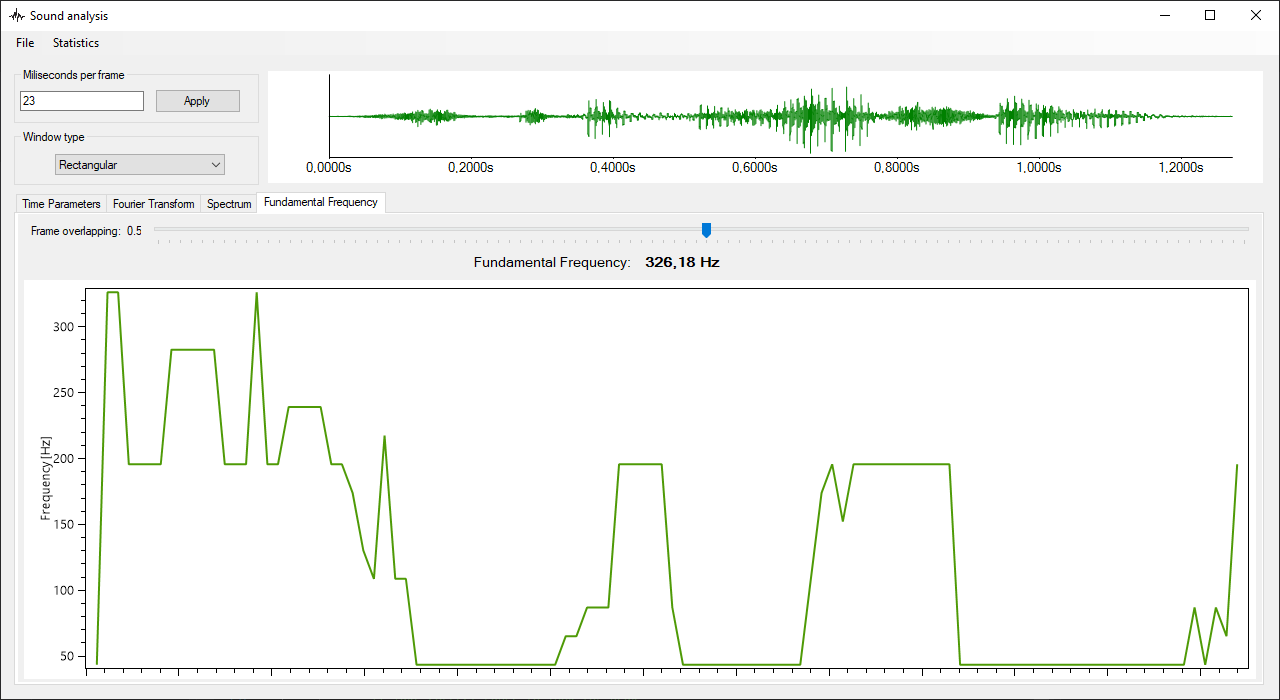
\includegraphics[width=0.86\linewidth]{images/15frequencyBro.png}
  \caption{Transformata Fouriera dla nagrania Pawła}
\end{figure}

\section{Wnioski}
Przeprowadzona analiza w jasny sposób potwierdza przydatność analizy nagrań audio w dziedzinie częstotliwości. Wyliczone parametry są szczególnie przydatne jeśli chodzi o wykrywanie dominujących częstotliwości, a co za tym idzie detekcję mowa-muzyka w obrębie jednego nagrania.\\
Warto tutaj odnieść się do wyników poprzedniego projektu, gdzie analiza w dziedzinie czasu nie dawała tak dokładnych wyników, a wiele fragmentów cichej mowy zlewało się wówczas z szumami czy też ciszą. W przypadku analizy w dziedzinie częstotliwości odróżnienie szumów od mowy jest zadaniem łatwym, w którym dodatkowo pomocne okazują się funkcje okienkowe.\\
Przeprowadzone eksperymenty pokazały również różnice w tonie podstawowym między wypowiedziami dwóch różnych osób, nawet takich o podobnym głosie. Jednak aby te wyniki brać na bieżąco należy dokładnie skupić się na sposobie i dynamice wypowiadania nagranej kwestii. Nie bez znaczenia jest także mikrofon - normalizacja nie zawsze jest w stanie zniwelować różnice wynikające z jego charakterystyki.

%\begin{figure}
%\centering
%\makebox[\textwidth][c]{
%\subfloat[Transformata Fouriera dla mojego nagrania]
%  {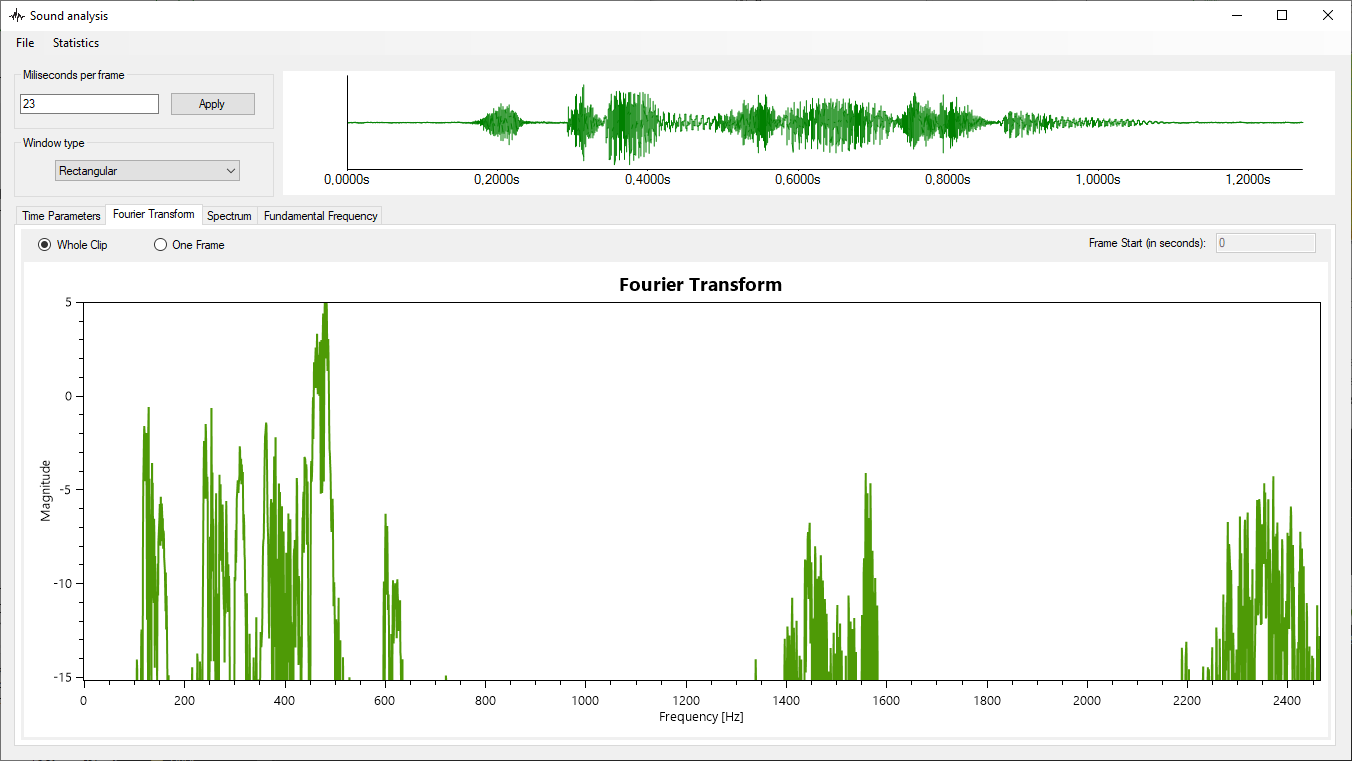
\includegraphics[width=0.55\textwidth]{images/10fourierMy.png}}
%\quad
%\subfloat[Transformata Fouriera dla nagrania brata]
%  {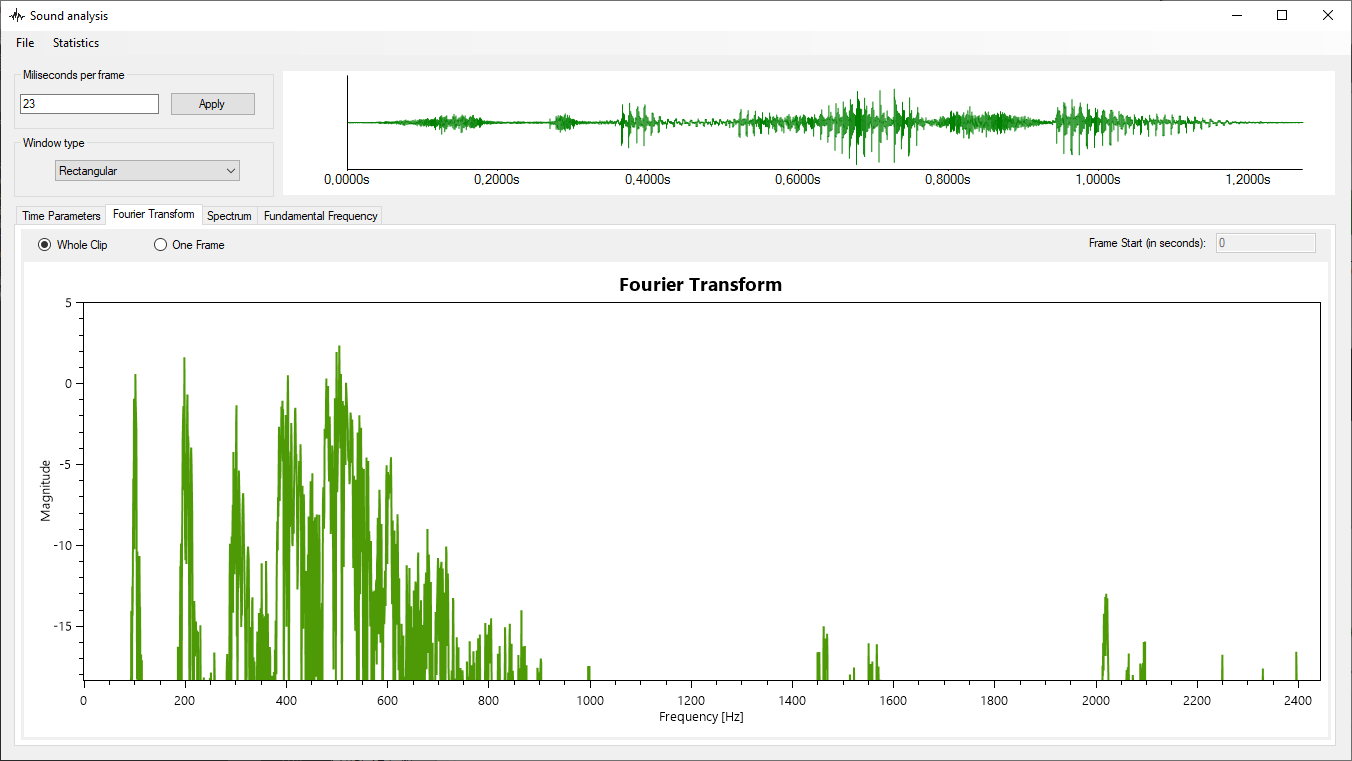
\includegraphics[width=0.55\textwidth]{images/11fourierBro.png}}
%\quad}%
%\end{figure}

%\lstset{basicstyle=\ttfamily}
%\lstset{style=sharpc}
%\begin{lstlisting}
%\end{lstlisting}

\end{document}